We examine the accuracy of the asymptotic approximations in Theorem \ref{thm:1} in finite samples, and of the correction by minimum calibration number introduced in Section \ref{sec:finite-sample}, via numerical simulation.

\subsection{Power as a function of the sample sizes}

We compare the theoretical predictions with empirical power of the following tests
\begin{itemize}
    \item Fisher's exact test
    \item Welch's t-test
    \item Pearson's chi-square test
    \item Likelihood ratio test, and 
    \item LR test with logistic regression.
\end{itemize}
Theses tests are performed on data simulated from the two-binomial model at following ranges of parameter values:
\begin{itemize}
    \item Sample size total, $n$: $100, 150, 200, 300, \ldots, 900, 1000, 1500, 2000, \ldots$, up to $10^5$,
    \item Fraction of cases in the study, $\phi$: $15\%$, $25\%$, $35\%$, $50\%$, $85\%$,
    \item Risk allele frequencies in the control group, $f$: $0.01\%$, $0.1\%$, $1\%$, $10\%$, $50\%$, $90\%$,
    \item Odds ratio, $R$: $1.05$, $1.1$, $1.2$, $1.5$, $3.0$.
    \item p-value cutoffs: $5\times 10^{-5}$, $5\times 10^{-8}$.
\end{itemize}
Each of the $41\times5\times6\times5\times2$ parameter value combinations was simulated $200$ times.
In the interest of space, only the results for p-value cutoff at $5\times 10^{-8}$, and odds ratios $1.05, 1.1, 1.5$ are visualized.
The figures are organized by increasing fraction of cases in the study $\phi$, in Figures \ref{fig:compare-phi015} to \ref{fig:compare-phi085}.

Each design (and test) were examined under small to moderate odds ratios (left to right panels), and under rare to common risk allele frequencies (top to bottom panels).
The Fisher's exact test (black circles), Welch's t-test (red triangles), Pearson's chi-square test (blue crosses), Likelihood ratio test, and equivalently, LR test with logistic regression (light blue diamonds) are compared against the theoretical predictions (purple nabla).

The accuracy of the theoretical predictions will be commented in Section \ref{subsec:accuracy-of-asymptotics}.

\iffalse
\begin{figure*}[!tpb]
\centering
        \subfigure{%
            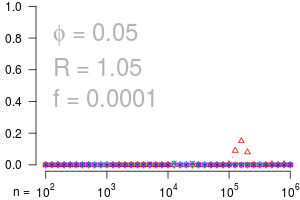
\includegraphics[width=0.26\textwidth]{simulation_plots/compare_tests/phi=005_R=105_f=1e-04.png}
        }%
        \subfigure{%
            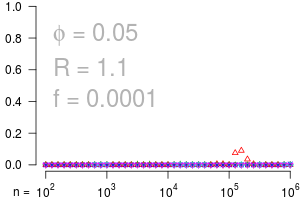
\includegraphics[width=0.26\textwidth]{simulation_plots/compare_tests/phi=005_R=110_f=1e-04.png}
        }%
        \subfigure{%
            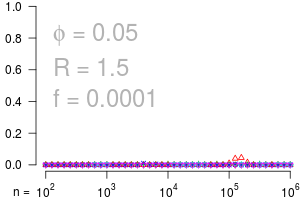
\includegraphics[width=0.26\textwidth]{simulation_plots/compare_tests/phi=005_R=150_f=1e-04.png}
        }\\ %  ------- End of the first row ----------------------%
        \subfigure{%
           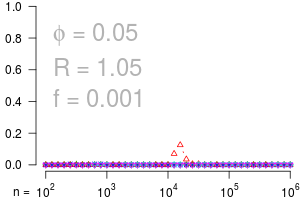
\includegraphics[width=0.26\textwidth]{simulation_plots/compare_tests/phi=005_R=105_f=0001.png}
        }%
        \subfigure{%
           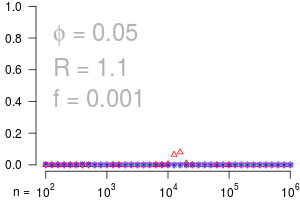
\includegraphics[width=0.26\textwidth]{simulation_plots/compare_tests/phi=005_R=110_f=0001.png}
        }%
        \subfigure{%
           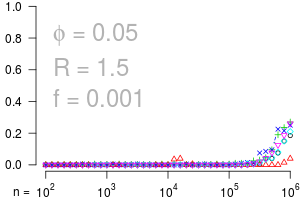
\includegraphics[width=0.26\textwidth]{simulation_plots/compare_tests/phi=005_R=150_f=0001.png}
        }\\ %  ------- End of the second row ----------------------%
        \subfigure{%
            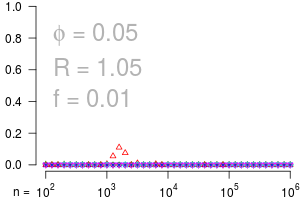
\includegraphics[width=0.26\textwidth]{simulation_plots/compare_tests/phi=005_R=105_f=001.png}
        }%
        \subfigure{%
            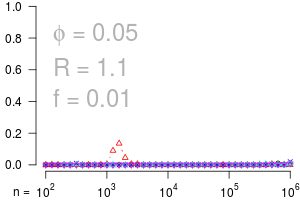
\includegraphics[width=0.26\textwidth]{simulation_plots/compare_tests/phi=005_R=110_f=001.png}
        }%
        \subfigure{%
            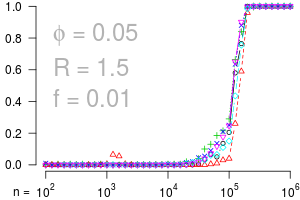
\includegraphics[width=0.26\textwidth]{simulation_plots/compare_tests/phi=005_R=150_f=001.png}
        }\\ %  ------- End of the third row ----------------------%
        \subfigure{%
            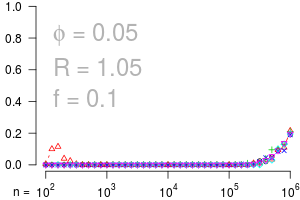
\includegraphics[width=0.26\textwidth]{simulation_plots/compare_tests/phi=005_R=105_f=01.png}
        }%
        \subfigure{%
            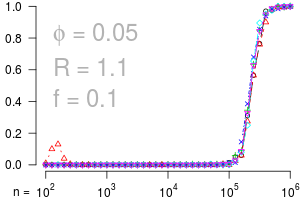
\includegraphics[width=0.26\textwidth]{simulation_plots/compare_tests/phi=005_R=110_f=01.png}
        }%
        \subfigure{%
            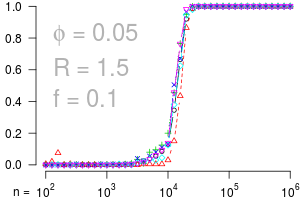
\includegraphics[width=0.26\textwidth]{simulation_plots/compare_tests/phi=005_R=150_f=01.png}
        }\\ %  ------- End of the fourth row ----------------------%
        \subfigure{%
            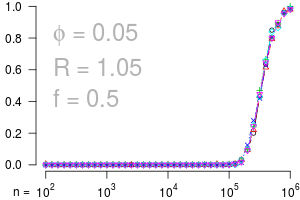
\includegraphics[width=0.26\textwidth]{simulation_plots/compare_tests/phi=005_R=105_f=05.png}
        }%
        \subfigure{%
            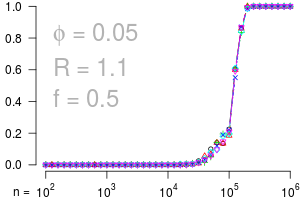
\includegraphics[width=0.26\textwidth]{simulation_plots/compare_tests/phi=005_R=110_f=05.png}
        }%
        \subfigure{%
            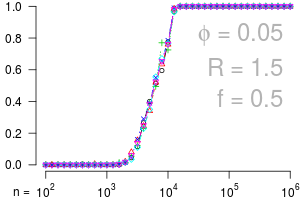
\includegraphics[width=0.26\textwidth]{simulation_plots/compare_tests/phi=005_R=150_f=05.png}
        }\\ %  ------- End of the fifth row ----------------------%
        \subfigure{%
            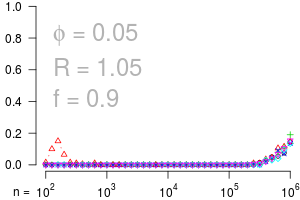
\includegraphics[width=0.26\textwidth]{simulation_plots/compare_tests/phi=005_R=105_f=09.png}
        }%
        \subfigure{%
            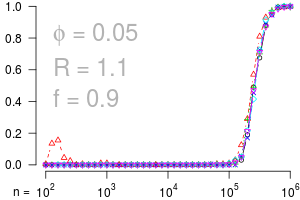
\includegraphics[width=0.26\textwidth]{simulation_plots/compare_tests/phi=005_R=110_f=09.png}
        }%
        \subfigure{%
            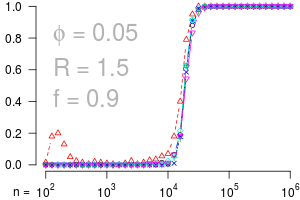
\includegraphics[width=0.26\textwidth]{simulation_plots/compare_tests/phi=005_R=150_f=09.png}
        }%
\caption{Empirical power as a function of sample sizes, under small to moderate odds ratios (left to right panels), and under rare to common risk allele frequencies (top to bottom panels).
The Fisher's exact test (black circles), Welch's t-test (red triangles), Pearson's chi-square test (blue crosses), Likelihood ratio test, and equivalently, LR test with logistic regression (light blue diamonds) are almost identical to the theoretical predictions (purple nabla), at sample sizes ranging from 100 to 100,000. Fraction of cases $\phi = 5\%$.
}\label{fig:compare-phi005}
\end{figure*}
\fi


\begin{figure*}[!tpb]
\centering
        \subfigure{%
            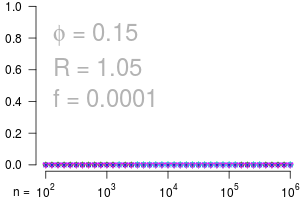
\includegraphics[width=0.26\textwidth]{simulation_plots/compare_tests/phi=015_R=105_f=1e-04.png}
        }%
        \subfigure{%
            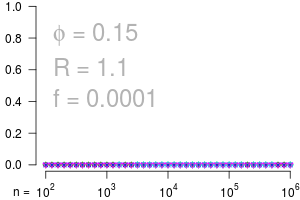
\includegraphics[width=0.26\textwidth]{simulation_plots/compare_tests/phi=015_R=110_f=1e-04.png}
        }%
        \subfigure{%
            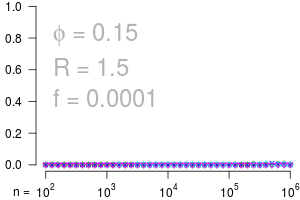
\includegraphics[width=0.26\textwidth]{simulation_plots/compare_tests/phi=015_R=150_f=1e-04.png}
        }\\ %  ------- End of the first row ----------------------%
        \subfigure{%
           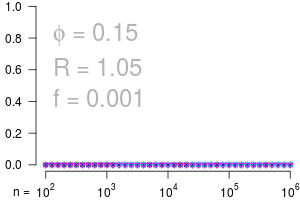
\includegraphics[width=0.26\textwidth]{simulation_plots/compare_tests/phi=015_R=105_f=0001.png}
        }%
        \subfigure{%
           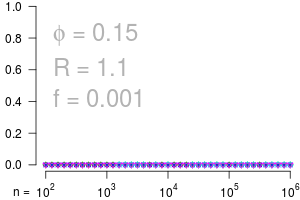
\includegraphics[width=0.26\textwidth]{simulation_plots/compare_tests/phi=015_R=110_f=0001.png}
        }%
        \subfigure{%
           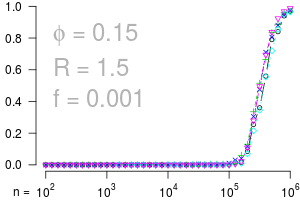
\includegraphics[width=0.26\textwidth]{simulation_plots/compare_tests/phi=015_R=150_f=0001.png}
        }\\ %  ------- End of the second row ----------------------%
        \subfigure{%
            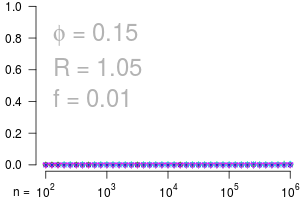
\includegraphics[width=0.26\textwidth]{simulation_plots/compare_tests/phi=015_R=105_f=001.png}
        }%
        \subfigure{%
            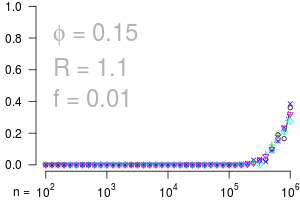
\includegraphics[width=0.26\textwidth]{simulation_plots/compare_tests/phi=015_R=110_f=001.png}
        }%
        \subfigure{%
            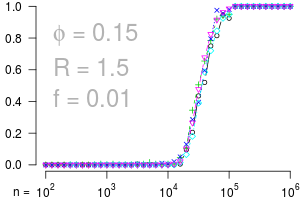
\includegraphics[width=0.26\textwidth]{simulation_plots/compare_tests/phi=015_R=150_f=001.png}
        }\\ %  ------- End of the third row ----------------------%
        \subfigure{%
            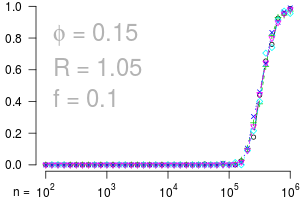
\includegraphics[width=0.26\textwidth]{simulation_plots/compare_tests/phi=015_R=105_f=01.png}
        }%
        \subfigure{%
            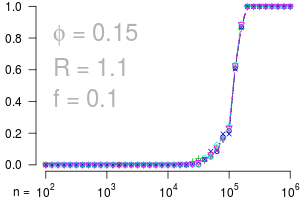
\includegraphics[width=0.26\textwidth]{simulation_plots/compare_tests/phi=015_R=110_f=01.png}
        }%
        \subfigure{%
            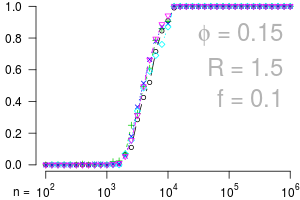
\includegraphics[width=0.26\textwidth]{simulation_plots/compare_tests/phi=015_R=150_f=01.png}
        }\\ %  ------- End of the fourth row ----------------------%
        \subfigure{%
            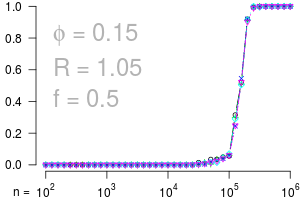
\includegraphics[width=0.26\textwidth]{simulation_plots/compare_tests/phi=015_R=105_f=05.png}
        }%
        \subfigure{%
            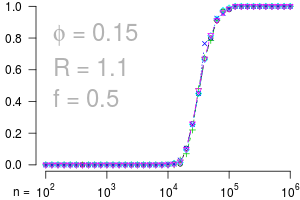
\includegraphics[width=0.26\textwidth]{simulation_plots/compare_tests/phi=015_R=110_f=05.png}
        }%
        \subfigure{%
            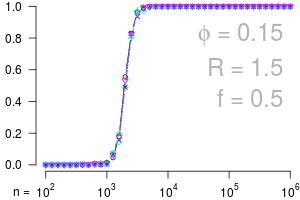
\includegraphics[width=0.26\textwidth]{simulation_plots/compare_tests/phi=015_R=150_f=05.png}
        }\\ %  ------- End of the fifth row ----------------------%
        \subfigure{%
            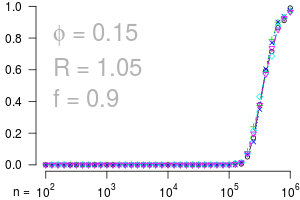
\includegraphics[width=0.26\textwidth]{simulation_plots/compare_tests/phi=015_R=105_f=09.png}
        }%
        \subfigure{%
            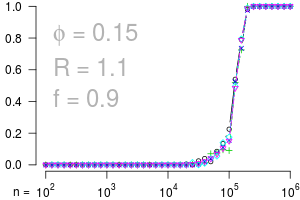
\includegraphics[width=0.26\textwidth]{simulation_plots/compare_tests/phi=015_R=110_f=09.png}
        }%
        \subfigure{%
            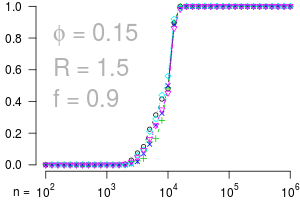
\includegraphics[width=0.26\textwidth]{simulation_plots/compare_tests/phi=015_R=150_f=09.png}
        }%
\caption{Empirical power as a function of sample sizes, under small to moderate odds ratios (left to right panels), and under rare to common risk allele frequencies (top to bottom panels).
The Fisher's exact test (black circles), Welch's t-test (red triangles), Pearson's chi-square test (blue crosses), Likelihood ratio test, and equivalently, LR test with logistic regression (light blue diamonds) are almost identical to the theoretical predictions (purple nabla), at sample sizes ranging from 100 to 100,000. Fraction of cases $\phi = 15\%$.
}\label{fig:compare-phi015}
\end{figure*}


\begin{figure*}[!tpb]
\centering
        \subfigure{%
            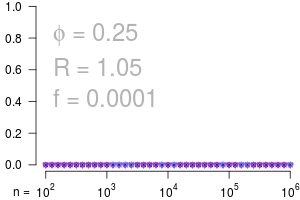
\includegraphics[width=0.26\textwidth]{simulation_plots/compare_tests/phi=025_R=105_f=1e-04.png}
        }%
        \subfigure{%
            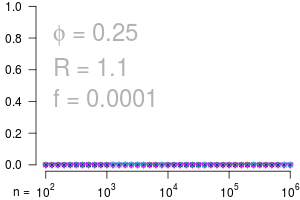
\includegraphics[width=0.26\textwidth]{simulation_plots/compare_tests/phi=025_R=110_f=1e-04.png}
        }%
        \subfigure{%
            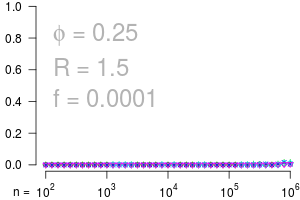
\includegraphics[width=0.26\textwidth]{simulation_plots/compare_tests/phi=025_R=150_f=1e-04.png}
        }\\ %  ------- End of the first row ----------------------%
        \subfigure{%
           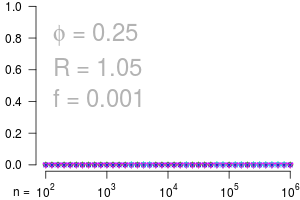
\includegraphics[width=0.26\textwidth]{simulation_plots/compare_tests/phi=025_R=105_f=0001.png}
        }%
        \subfigure{%
           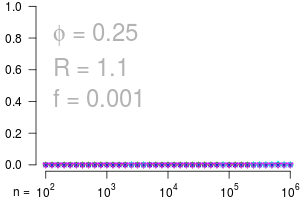
\includegraphics[width=0.26\textwidth]{simulation_plots/compare_tests/phi=025_R=110_f=0001.png}
        }%
        \subfigure{%
           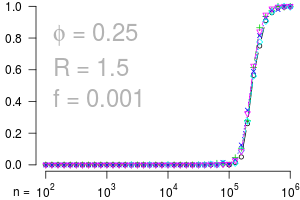
\includegraphics[width=0.26\textwidth]{simulation_plots/compare_tests/phi=025_R=150_f=0001.png}
        }\\ %  ------- End of the second row ----------------------%
        \subfigure{%
            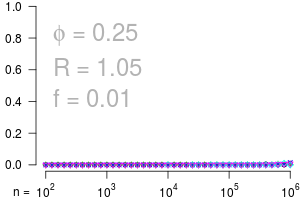
\includegraphics[width=0.26\textwidth]{simulation_plots/compare_tests/phi=025_R=105_f=001.png}
        }%
        \subfigure{%
            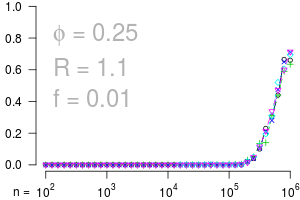
\includegraphics[width=0.26\textwidth]{simulation_plots/compare_tests/phi=025_R=110_f=001.png}
        }%
        \subfigure{%
            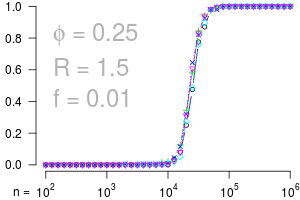
\includegraphics[width=0.26\textwidth]{simulation_plots/compare_tests/phi=025_R=150_f=001.png}
        }\\ %  ------- End of the third row ----------------------%
        \subfigure{%
            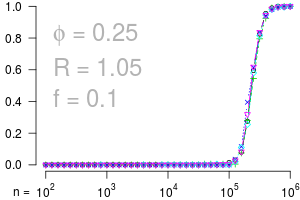
\includegraphics[width=0.26\textwidth]{simulation_plots/compare_tests/phi=025_R=105_f=01.png}
        }%
        \subfigure{%
            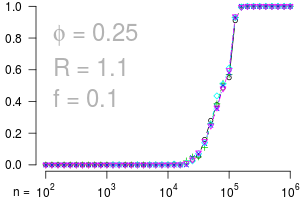
\includegraphics[width=0.26\textwidth]{simulation_plots/compare_tests/phi=025_R=110_f=01.png}
        }%
        \subfigure{%
            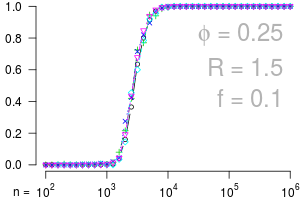
\includegraphics[width=0.26\textwidth]{simulation_plots/compare_tests/phi=025_R=150_f=01.png}
        }\\ %  ------- End of the fourth row ----------------------%
        \subfigure{%
            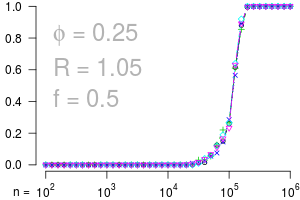
\includegraphics[width=0.26\textwidth]{simulation_plots/compare_tests/phi=025_R=105_f=05.png}
        }%
        \subfigure{%
            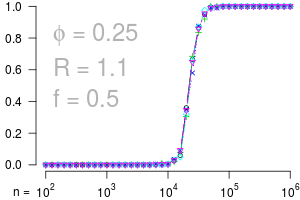
\includegraphics[width=0.26\textwidth]{simulation_plots/compare_tests/phi=025_R=110_f=05.png}
        }%
        \subfigure{%
            \includegraphics[width=0.26\textwidth]{simulation_plots/compare_tests/phi=025_R=150_f=05.png}
        }\\ %  ------- End of the fifth row ----------------------%
        \subfigure{%
            \includegraphics[width=0.26\textwidth]{simulation_plots/compare_tests/phi=025_R=105_f=09.png}
        }%
        \subfigure{%
            \includegraphics[width=0.26\textwidth]{simulation_plots/compare_tests/phi=025_R=110_f=09.png}
        }%
        \subfigure{%
            \includegraphics[width=0.26\textwidth]{simulation_plots/compare_tests/phi=025_R=150_f=09.png}
        }%
\caption{Empirical power as a function of sample sizes, under small to moderate odds ratios (left to right panels), and under rare to common risk allele frequencies (top to bottom panels).
The Fisher's exact test (black circles), Welch's t-test (red triangles), Pearson's chi-square test (blue crosses), Likelihood ratio test, and equivalently, LR test with logistic regression (light blue diamonds) are almost identical to the theoretical predictions (purple nabla), at sample sizes ranging from 100 to 100,000. Fraction of cases $\phi = 25\%$.
}\label{fig:compare-phi025}
\end{figure*}


\begin{figure*}[!tpb]
\centering
        \subfigure{%
            \includegraphics[width=0.26\textwidth]{simulation_plots/compare_tests/phi=035_R=105_f=1e-04.png}
        }%
        \subfigure{%
            \includegraphics[width=0.26\textwidth]{simulation_plots/compare_tests/phi=035_R=110_f=1e-04.png}
        }%
        \subfigure{%
            \includegraphics[width=0.26\textwidth]{simulation_plots/compare_tests/phi=035_R=150_f=1e-04.png}
        }\\ %  ------- End of the first row ----------------------%
        \subfigure{%
           \includegraphics[width=0.26\textwidth]{simulation_plots/compare_tests/phi=035_R=105_f=0001.png}
        }%
        \subfigure{%
           \includegraphics[width=0.26\textwidth]{simulation_plots/compare_tests/phi=035_R=110_f=0001.png}
        }%
        \subfigure{%
           \includegraphics[width=0.26\textwidth]{simulation_plots/compare_tests/phi=035_R=150_f=0001.png}
        }\\ %  ------- End of the second row ----------------------%
        \subfigure{%
            \includegraphics[width=0.26\textwidth]{simulation_plots/compare_tests/phi=035_R=105_f=001.png}
        }%
        \subfigure{%
            \includegraphics[width=0.26\textwidth]{simulation_plots/compare_tests/phi=035_R=110_f=001.png}
        }%
        \subfigure{%
            \includegraphics[width=0.26\textwidth]{simulation_plots/compare_tests/phi=035_R=150_f=001.png}
        }\\ %  ------- End of the third row ----------------------%
        \subfigure{%
            \includegraphics[width=0.26\textwidth]{simulation_plots/compare_tests/phi=035_R=105_f=01.png}
        }%
        \subfigure{%
            \includegraphics[width=0.26\textwidth]{simulation_plots/compare_tests/phi=035_R=110_f=01.png}
        }%
        \subfigure{%
            \includegraphics[width=0.26\textwidth]{simulation_plots/compare_tests/phi=035_R=150_f=01.png}
        }\\ %  ------- End of the fourth row ----------------------%
        \subfigure{%
            \includegraphics[width=0.26\textwidth]{simulation_plots/compare_tests/phi=035_R=105_f=05.png}
        }%
        \subfigure{%
            \includegraphics[width=0.26\textwidth]{simulation_plots/compare_tests/phi=035_R=110_f=05.png}
        }%
        \subfigure{%
            \includegraphics[width=0.26\textwidth]{simulation_plots/compare_tests/phi=035_R=150_f=05.png}
        }\\ %  ------- End of the fifth row ----------------------%
        \subfigure{%
            \includegraphics[width=0.26\textwidth]{simulation_plots/compare_tests/phi=035_R=105_f=09.png}
        }%
        \subfigure{%
            \includegraphics[width=0.26\textwidth]{simulation_plots/compare_tests/phi=035_R=110_f=09.png}
        }%
        \subfigure{%
            \includegraphics[width=0.26\textwidth]{simulation_plots/compare_tests/phi=035_R=150_f=09.png}
        }%
\caption{Empirical power as a function of sample sizes, under small to moderate odds ratios (left to right panels), and under rare to common risk allele frequencies (top to bottom panels).
The Fisher's exact test (black circles), Welch's t-test (red triangles), Pearson's chi-square test (blue crosses), Likelihood ratio test, and equivalently, LR test with logistic regression (light blue diamonds) are almost identical to the theoretical predictions (purple nabla), at sample sizes ranging from 100 to 100,000. Fraction of cases $\phi = 35\%$.
}\label{fig:compare-phi035}
\end{figure*}


\begin{figure*}[!tpb]
\centering
        \subfigure{%
            \includegraphics[width=0.26\textwidth]{simulation_plots/compare_tests/phi=050_R=105_f=1e-04.png}
        }%
        \subfigure{%
            \includegraphics[width=0.26\textwidth]{simulation_plots/compare_tests/phi=050_R=110_f=1e-04.png}
        }%
        \subfigure{%
            \includegraphics[width=0.26\textwidth]{simulation_plots/compare_tests/phi=050_R=150_f=1e-04.png}
        }\\ %  ------- End of the first row ----------------------%
        \subfigure{%
           \includegraphics[width=0.26\textwidth]{simulation_plots/compare_tests/phi=050_R=105_f=0001.png}
        }%
        \subfigure{%
           \includegraphics[width=0.26\textwidth]{simulation_plots/compare_tests/phi=050_R=110_f=0001.png}
        }%
        \subfigure{%
           \includegraphics[width=0.26\textwidth]{simulation_plots/compare_tests/phi=050_R=150_f=0001.png}
        }\\ %  ------- End of the second row ----------------------%
        \subfigure{%
            \includegraphics[width=0.26\textwidth]{simulation_plots/compare_tests/phi=050_R=105_f=001.png}
        }%
        \subfigure{%
            \includegraphics[width=0.26\textwidth]{simulation_plots/compare_tests/phi=050_R=110_f=001.png}
        }%
        \subfigure{%
            \includegraphics[width=0.26\textwidth]{simulation_plots/compare_tests/phi=050_R=150_f=001.png}
        }\\ %  ------- End of the third row ----------------------%
        \subfigure{%
            \includegraphics[width=0.26\textwidth]{simulation_plots/compare_tests/phi=050_R=105_f=01.png}
        }%
        \subfigure{%
            \includegraphics[width=0.26\textwidth]{simulation_plots/compare_tests/phi=050_R=110_f=01.png}
        }%
        \subfigure{%
            \includegraphics[width=0.26\textwidth]{simulation_plots/compare_tests/phi=050_R=150_f=01.png}
        }\\ %  ------- End of the fourth row ----------------------%
        \subfigure{%
            \includegraphics[width=0.26\textwidth]{simulation_plots/compare_tests/phi=050_R=105_f=05.png}
        }%
        \subfigure{%
            \includegraphics[width=0.26\textwidth]{simulation_plots/compare_tests/phi=050_R=110_f=05.png}
        }%
        \subfigure{%
            \includegraphics[width=0.26\textwidth]{simulation_plots/compare_tests/phi=050_R=150_f=05.png}
        }\\ %  ------- End of the fifth row ----------------------%
        \subfigure{%
            \includegraphics[width=0.26\textwidth]{simulation_plots/compare_tests/phi=050_R=105_f=09.png}
        }%
        \subfigure{%
            \includegraphics[width=0.26\textwidth]{simulation_plots/compare_tests/phi=050_R=110_f=09.png}
        }%
        \subfigure{%
            \includegraphics[width=0.26\textwidth]{simulation_plots/compare_tests/phi=050_R=150_f=09.png}
        }%
\caption{Empirical power as a function of sample sizes, under small to moderate odds ratios (left to right panels), and under rare to common risk allele frequencies (top to bottom panels).
The Fisher's exact test (black circles), Welch's t-test (red triangles), Pearson's chi-square test (blue crosses), Likelihood ratio test, and equivalently, LR test with logistic regression (light blue diamonds) are almost identical to the theoretical predictions (purple nabla), at sample sizes ranging from 100 to 100,000. Fraction of cases $\phi = 50\%$.
}\label{fig:compare-phi050}
\end{figure*}


\begin{figure*}[!tpb]
\centering
        \subfigure{%
            \includegraphics[width=0.26\textwidth]{simulation_plots/compare_tests/phi=085_R=105_f=1e-04.png}
        }%
        \subfigure{%
            \includegraphics[width=0.26\textwidth]{simulation_plots/compare_tests/phi=085_R=110_f=1e-04.png}
        }%
        \subfigure{%
            \includegraphics[width=0.26\textwidth]{simulation_plots/compare_tests/phi=085_R=150_f=1e-04.png}
        }\\ %  ------- End of the first row ----------------------%
        \subfigure{%
           \includegraphics[width=0.26\textwidth]{simulation_plots/compare_tests/phi=085_R=105_f=0001.png}
        }%
        \subfigure{%
           \includegraphics[width=0.26\textwidth]{simulation_plots/compare_tests/phi=085_R=110_f=0001.png}
        }%
        \subfigure{%
           \includegraphics[width=0.26\textwidth]{simulation_plots/compare_tests/phi=085_R=150_f=0001.png}
        }\\ %  ------- End of the second row ----------------------%
        \subfigure{%
            \includegraphics[width=0.26\textwidth]{simulation_plots/compare_tests/phi=085_R=105_f=001.png}
        }%
        \subfigure{%
            \includegraphics[width=0.26\textwidth]{simulation_plots/compare_tests/phi=085_R=110_f=001.png}
        }%
        \subfigure{%
            \includegraphics[width=0.26\textwidth]{simulation_plots/compare_tests/phi=085_R=150_f=001.png}
        }\\ %  ------- End of the third row ----------------------%
        \subfigure{%
            \includegraphics[width=0.26\textwidth]{simulation_plots/compare_tests/phi=085_R=105_f=01.png}
        }%
        \subfigure{%
            \includegraphics[width=0.26\textwidth]{simulation_plots/compare_tests/phi=085_R=110_f=01.png}
        }%
        \subfigure{%
            \includegraphics[width=0.26\textwidth]{simulation_plots/compare_tests/phi=085_R=150_f=01.png}
        }\\ %  ------- End of the fourth row ----------------------%
        \subfigure{%
            \includegraphics[width=0.26\textwidth]{simulation_plots/compare_tests/phi=085_R=105_f=05.png}
        }%
        \subfigure{%
            \includegraphics[width=0.26\textwidth]{simulation_plots/compare_tests/phi=085_R=110_f=05.png}
        }%
        \subfigure{%
            \includegraphics[width=0.26\textwidth]{simulation_plots/compare_tests/phi=085_R=150_f=05.png}
        }\\ %  ------- End of the fifth row ----------------------%
        \subfigure{%
            \includegraphics[width=0.26\textwidth]{simulation_plots/compare_tests/phi=085_R=105_f=09.png}
        }%
        \subfigure{%
            \includegraphics[width=0.26\textwidth]{simulation_plots/compare_tests/phi=085_R=110_f=09.png}
        }%
        \subfigure{%
            \includegraphics[width=0.26\textwidth]{simulation_plots/compare_tests/phi=085_R=150_f=09.png}
        }%
\caption{Empirical power as a function of sample sizes, under small to moderate odds ratios (left to right panels), and under rare to common risk allele frequencies (top to bottom panels).
The Fisher's exact test (black circles), Welch's t-test (red triangles), Pearson's chi-square test (blue crosses), Likelihood ratio test, and equivalently, LR test with logistic regression (light blue diamonds) are almost identical to the theoretical predictions (purple nabla), at sample sizes ranging from 100 to 100,000. Fraction of cases $\phi = 85\%$.
}\label{fig:compare-phi085}
\end{figure*}

\subsection{Power as a function of the canonical parameters}

To fully explore the accuracy of the theoretical predictions, we extend the simulation to a wider range of model parameters.
\begin{itemize}
    \item Sample size total, $n$: $10^2$, $10^3$, $10^4$, $10^5$,
    \item Fraction of cases in the study, $\phi$: $5\%$, $15\%$, $25\%$ $50\%$, $85\%$,
    \item Risk allele frequencies in control group, $f$: a grid of $100$ values ranging from $0.01\%$ to $99.5\%$. The values are non-regularly spaced; more values are selected towards the end points of the interval $(0,1)$.
    \item Odds ratio, $R$: a grid of $100$ values ranging from $1$ to $100$. The values are regularly spaced on the log-scale.
    \item p-value cutoffs: $5\times 10^{-5}$, $5\times 10^{-8}$.
\end{itemize}
Each of the $4\times4\times100\times100\times2$ parameter value combinations were simulated $1000$ times.

We compare the theoretical results with powers of Fisher's exact test obtained by simulations.
We choose to compare against exact tests for their superior performance in finite samples ---
while approximate tests like the chi-square test and likelihood ratio tests may fail to protect against type I error inflation when sample sizes are small, exact tests maintain the correct levels. 

The results for p-value cutoff at $5\times 10^{-8}$ are visualized in the form ``OR-RAF diagrams'' to better highlight settings under which the theoretical predictions and the empirical powers differ.

\begin{figure*}[!tpb]%figure1
\centering
        \subfigure{%
            \includegraphics[width=0.30\textwidth]{simulation_plots/phase_diagram/n100_phi005_p5e-8_theoretical.png}
        }%
        \subfigure{%
           \includegraphics[width=0.30\textwidth]{simulation_plots/phase_diagram/n100_phi005_p5e-8.png}
        }%
        \subfigure{%
            \includegraphics[width=0.30\textwidth]{simulation_plots/phase_diagram/n100_phi005_p5e-8_diff.png}
        } \\ %  ------- End of the first row ----------------------%
        \subfigure{%
            \includegraphics[width=0.30\textwidth]{simulation_plots/phase_diagram/n1000_phi005_p5e-8_theoretical.png}
        }%
        \subfigure{%
            \includegraphics[width=0.30\textwidth]{simulation_plots/phase_diagram/n1000_phi005_p5e-8.png}
        }%
        \subfigure{%
            \includegraphics[width=0.30\textwidth]{simulation_plots/phase_diagram/n1000_phi005_p5e-8_diff.png}
        } \\ %  ------- End of the second row ----------------------%
        \subfigure{%
            \includegraphics[width=0.30\textwidth]{simulation_plots/phase_diagram/n10000_phi005_p5e-8_theoretical.png}
        }%
        \subfigure{%
            \includegraphics[width=0.30\textwidth]{simulation_plots/phase_diagram/n10000_phi005_p5e-8.png}
        }%
        \subfigure{%
            \includegraphics[width=0.30\textwidth]{simulation_plots/phase_diagram/n10000_phi005_p5e-8_diff.png}
        } \\ %  ------- End of the third row ----------------------%
        \subfigure{%
            \includegraphics[width=0.30\textwidth]{simulation_plots/phase_diagram/n100000_phi005_p5e-8_theoretical.png}
        }%
        \subfigure{%
            \includegraphics[width=0.30\textwidth]{simulation_plots/phase_diagram/n100000_phi005_p5e-8.png}
        }%
        \subfigure{%
            \includegraphics[width=0.30\textwidth]{simulation_plots/phase_diagram/n100000_phi005_p5e-8_diff.png}
        }
\caption{
Statistical powers for the OR-RAF combinations, obtained from theoretical predictions (left column) and by simulations (middle column). Their absolute differences (right column) are shown at sample sizes ranging from $100$ to $100,000$ (top to bottom).
p-value threshold is at $5\times10^{-8}$.
Fractions of cases $\phi=5\%$.
}\label{fig:phi005}
\end{figure*}

\begin{figure*}[!tpb]%figure1
\centering
        \subfigure{%
            \includegraphics[width=0.30\textwidth]{simulation_plots/phase_diagram/n100_phi015_p5e-8_theoretical.png}
        }%
        \subfigure{%
           \includegraphics[width=0.30\textwidth]{simulation_plots/phase_diagram/n100_phi015_p5e-8.png}
        }%
        \subfigure{%
            \includegraphics[width=0.30\textwidth]{simulation_plots/phase_diagram/n100_phi015_p5e-8_diff.png}
        } \\ %  ------- End of the first row ----------------------%
        \subfigure{%
            \includegraphics[width=0.30\textwidth]{simulation_plots/phase_diagram/n1000_phi015_p5e-8_theoretical.png}
        }%
        \subfigure{%
            \includegraphics[width=0.30\textwidth]{simulation_plots/phase_diagram/n1000_phi015_p5e-8.png}
        }%
        \subfigure{%
            \includegraphics[width=0.30\textwidth]{simulation_plots/phase_diagram/n1000_phi015_p5e-8_diff.png}
        } \\ %  ------- End of the second row ----------------------%
        \subfigure{%
            \includegraphics[width=0.30\textwidth]{simulation_plots/phase_diagram/n10000_phi015_p5e-8_theoretical.png}
        }%
        \subfigure{%
            \includegraphics[width=0.30\textwidth]{simulation_plots/phase_diagram/n10000_phi015_p5e-8.png}
        }%
        \subfigure{%
            \includegraphics[width=0.30\textwidth]{simulation_plots/phase_diagram/n10000_phi015_p5e-8_diff.png}
        } \\ %  ------- End of the third row ----------------------%
        \subfigure{%
            \includegraphics[width=0.30\textwidth]{simulation_plots/phase_diagram/n100000_phi015_p5e-8_theoretical.png}
        } %
        \subfigure{%
            \includegraphics[width=0.30\textwidth]{simulation_plots/phase_diagram/n100000_phi015_p5e-8.png}
        }%
        \subfigure{%
            \includegraphics[width=0.30\textwidth]{simulation_plots/phase_diagram/n100000_phi015_p5e-8_diff.png}
        } %
\caption{
Statistical powers for the OR-RAF combinations, obtained from theoretical predictions (left column) and by simulations (middle column). Their absolute differences (right column) are shown at sample sizes ranging from $100$ to $100,000$ (top to bottom).
p-value threshold is at $5\times10^{-8}$.
Fractions of cases $\phi=15\%$.
}\label{fig:phi015}
\end{figure*}

\begin{figure*}[!tpb]%figure1
\centering
        \subfigure{%
            \includegraphics[width=0.30\textwidth]{simulation_plots/phase_diagram/n100_phi025_p5e-8_theoretical.png}
        }%
        \subfigure{%
           \includegraphics[width=0.30\textwidth]{simulation_plots/phase_diagram/n100_phi025_p5e-8.png}
        }%
        \subfigure{%
            \includegraphics[width=0.30\textwidth]{simulation_plots/phase_diagram/n100_phi025_p5e-8_diff.png}
        } \\ %  ------- End of the first row ----------------------%
        \subfigure{%
            \includegraphics[width=0.30\textwidth]{simulation_plots/phase_diagram/n1000_phi025_p5e-8_theoretical.png}
        }%
        \subfigure{%
            \includegraphics[width=0.30\textwidth]{simulation_plots/phase_diagram/n1000_phi025_p5e-8.png}
        }%
        \subfigure{%
            \includegraphics[width=0.30\textwidth]{simulation_plots/phase_diagram/n1000_phi025_p5e-8_diff.png}
        } \\ %  ------- End of the second row ----------------------%
        \subfigure{%
            \includegraphics[width=0.30\textwidth]{simulation_plots/phase_diagram/n10000_phi025_p5e-8_theoretical.png}
        }%
        \subfigure{%
            \includegraphics[width=0.30\textwidth]{simulation_plots/phase_diagram/n10000_phi025_p5e-8.png}
        }%
        \subfigure{%
            \includegraphics[width=0.30\textwidth]{simulation_plots/phase_diagram/n10000_phi025_p5e-8_diff.png}
        } \\ %  ------- End of the third row ----------------------%
        \subfigure{%
            \includegraphics[width=0.30\textwidth]{simulation_plots/phase_diagram/n100000_phi025_p5e-8_theoretical.png}
        }%
        \subfigure{%
            \includegraphics[width=0.30\textwidth]{simulation_plots/phase_diagram/n100000_phi025_p5e-8.png}
        }%
        \subfigure{%
            \includegraphics[width=0.30\textwidth]{simulation_plots/phase_diagram/n100000_phi025_p5e-8_diff.png}
        } %
\caption{
Statistical powers for the OR-RAF combinations, obtained from theoretical predictions (left column) and by simulations (middle column). Their absolute differences (right column) are shown at sample sizes ranging from $100$ to $100,000$ (top to bottom).
p-value threshold is at $5\times10^{-8}$.
Fractions of cases $\phi=25\%$.
}\label{fig:phi025}
\end{figure*}


\begin{figure*}[!tpb]%figure1
\centering
        \subfigure{%
            \includegraphics[width=0.30\textwidth]{simulation_plots/phase_diagram/n100_phi05_p5e-8_theoretical.png}
        }%
        \subfigure{%
           \includegraphics[width=0.30\textwidth]{simulation_plots/phase_diagram/n100_phi05_p5e-8.png}
        }%
        \subfigure{%
            \includegraphics[width=0.30\textwidth]{simulation_plots/phase_diagram/n100_phi05_p5e-8_diff.png}
        } \\ %  ------- End of the first row ----------------------%
        \subfigure{%
            \includegraphics[width=0.30\textwidth]{simulation_plots/phase_diagram/n1000_phi05_p5e-8_theoretical.png}
        }%
        \subfigure{%
            \includegraphics[width=0.30\textwidth]{simulation_plots/phase_diagram/n1000_phi05_p5e-8.png}
        }%
        \subfigure{%
            \includegraphics[width=0.30\textwidth]{simulation_plots/phase_diagram/n1000_phi05_p5e-8_diff.png}
        } \\ %  ------- End of the second row ----------------------%
        \subfigure{%
            \includegraphics[width=0.30\textwidth]{simulation_plots/phase_diagram/n10000_phi05_p5e-8_theoretical.png}
        }%
        \subfigure{%
            \includegraphics[width=0.30\textwidth]{simulation_plots/phase_diagram/n10000_phi05_p5e-8.png}
        }%
        \subfigure{%
            \includegraphics[width=0.30\textwidth]{simulation_plots/phase_diagram/n10000_phi05_p5e-8_diff.png}
        } \\ %  ------- End of the third row ----------------------%
        \subfigure{%
            \includegraphics[width=0.30\textwidth]{simulation_plots/phase_diagram/n100000_phi05_p5e-8_theoretical.png}
        }%
        \subfigure{%
            \includegraphics[width=0.30\textwidth]{simulation_plots/phase_diagram/n100000_phi05_p5e-8.png}
        }%
        \subfigure{%
            \includegraphics[width=0.30\textwidth]{simulation_plots/phase_diagram/n100000_phi05_p5e-8_diff.png}
        }
\caption{
Statistical powers for the OR-RAF combinations, obtained from theoretical predictions (left column) and by simulations (middle column). Their absolute differences (right column) are shown at sample sizes ranging from $100$ to $100,000$ (top to bottom).
p-value threshold is at $5\times10^{-8}$.
Fractions of cases $\phi=50\%$.
}\label{fig:phi05}
\end{figure*}

\begin{figure*}[!tpb]%figure1
\centering
        \subfigure{%
            \includegraphics[width=0.30\textwidth]{simulation_plots/phase_diagram/n100_phi085_p5e-8_theoretical.png}
        }%
        \subfigure{%
           \includegraphics[width=0.30\textwidth]{simulation_plots/phase_diagram/n100_phi085_p5e-8.png}
        }%
        \subfigure{%
            \includegraphics[width=0.30\textwidth]{simulation_plots/phase_diagram/n100_phi085_p5e-8_diff.png}
        } \\ %  ------- End of the first row ----------------------%
        \subfigure{%
            \includegraphics[width=0.30\textwidth]{simulation_plots/phase_diagram/n1000_phi085_p5e-8_theoretical.png}
        }%
        \subfigure{%
            \includegraphics[width=0.30\textwidth]{simulation_plots/phase_diagram/n1000_phi085_p5e-8.png}
        }%
        \subfigure{%
            \includegraphics[width=0.30\textwidth]{simulation_plots/phase_diagram/n1000_phi085_p5e-8_diff.png}
        } \\ %  ------- End of the second row ----------------------%
        \subfigure{%
            \includegraphics[width=0.30\textwidth]{simulation_plots/phase_diagram/n10000_phi085_p5e-8_theoretical.png}
        }%
        \subfigure{%
            \includegraphics[width=0.30\textwidth]{simulation_plots/phase_diagram/n10000_phi085_p5e-8.png}
        }%
        \subfigure{%
            \includegraphics[width=0.30\textwidth]{simulation_plots/phase_diagram/n10000_phi085_p5e-8_diff.png}
        } \\ %  ------- End of the third row ----------------------%
        \subfigure{%
            \includegraphics[width=0.30\textwidth]{simulation_plots/phase_diagram/n100000_phi085_p5e-8_theoretical.png}
        }%
        \subfigure{%
            \includegraphics[width=0.30\textwidth]{simulation_plots/phase_diagram/n100000_phi085_p5e-8.png}
        }%
        \subfigure{%
            \includegraphics[width=0.30\textwidth]{simulation_plots/phase_diagram/n100000_phi085_p5e-8_diff.png}
        } %
\caption{
Statistical powers for the OR-RAF combinations, obtained from theoretical predictions (left column) and by simulations (middle column). Their absolute differences (right column) are shown at sample sizes ranging from $100$ to $100,000$ (top to bottom).
p-value threshold is at $5\times10^{-8}$.
Fractions of cases $\phi=85\%$.
}\label{fig:phi085}
\end{figure*}


The results are shown in Figures \ref{fig:phi005} to \ref{fig:phi085}, organized by increasing fraction of cases in the study $\phi$.
Left columns of the figures show the theoretical predictions obtained by Theorem \ref{thm:1}, the middle columns shows the estimated powers from simulation, and the right columns visualize their differences.
Sample sizes ranging from $100$ to $100,000$ are arranged from top to bottom in each figure.


\subsection{Accuracy of theoretical predictions}
\label{subsec:accuracy-of-asymptotics}

% We now comment on some major features of the theoretical predictions.

We find that the asymptotic approximations in Theorem \ref{thm:1} to be robust for small to moderate odds ratios ($R<2$), as seen in all simulation studies (see Figures \ref{fig:compare-phi015} to \ref{fig:phi085}).

The theoretical approximations are extremely accurate (within 1 percentage point in absolute deviations) for balanced designs, even at very small sample sizes (see Figure \ref{fig:phi05}), as well as in settings with moderately more controls than controls at large sample sizes (see Figures \ref{fig:phi015} and \ref{fig:phi025}, $n=100,000$).
Some discrepancies can be seen under designs with too few cases (see Figure \ref{fig:phi005}) as well as too few controls (see Figure \ref{fig:phi085}), although the differences vanish as the sample sizes increase.

\begin{table}[h]
\begin{center}
    \begin{tabular}{cccccc}
    \hline
        & \multicolumn{5}{c}{Fraction of cases $\phi$} \\
        \cline{2-6}
        sample size $n$ & $5\%$ & $15\%$ & $25\%$ & $50\%$ & $85\%$ \\
        \hline
        $100$ & 4.61 (0.15) & 2.39 (0.08) & 1.44 (0.05) & 0.78 (0.02) & 2.00 (0.07) \\
        $1,000$ & 5.01 (0.15) & 3.37 (0.10) & 2.35 (0.7) & 1.03 (0.03) & 3.44 (0.10) \\
        $10,000$ & 4.73 (0.14) & 3.06 (0.09) & 1.98 (0.07) & 0.50 (0.02) & 2.43 (0.08) \\
        $100,000$ & 1.74 (0.07) & 0.73 (0.03) & 0.43 (0.02) & 0.18 (0.01) & 0.88 (0.04) \\
    \hline
    \end{tabular}
    \caption{Mean absolute deviations in percentage points between the theoretical predictions and the simulated results, with standard errors in brackets. The p-values threshold are set at $5\times10^{-8}$.}
    \label{tbl:accuracy-of-asymptotic-power}
\end{center}
\end{table}


In general, the mismatch between the theoretical predictions and empirical power only takes place at small sample sizes, and only for large odds ratios ($R>3$).
% The proposed correction based on minimum calibration numbers seems to provide a simple resolution for this mismatch.
% Alternatives with expected allele counts less than required by the minimum calibration numbers (outside the red dashed lines) should be interpreted to have near zero power.
% That is, in the OR-RAF diagrams, regions outside the red dashed lines should also be colored dark.
% The corrected predictions are closer to what is obtained for exact tests.
For small odds ratios, numerical experiments suggest that our power calculations are robust across a wide range of case-control ratios and sample sizes.

Theoretical predictions for p-value cutoff at $5\times 10^{-5}$ are up to $20\%$ more accurate than for p-value cutoff at $5\times 10^{-8}$, but qualitatively similar.
For example, the average absolute deviation for unbalanced designs ($\phi=15\%$) at sample size $n=100,000$ is only $0.57$ percentage points for p-value cutoff at $5\times 10^{-5}$, down from $0.73$ percentage points when p-value cutoff is at $5\times 10^{-8}$.
The same metric improves to $0.16$, down from $0.18$ percentage points, for balanced designs ($\phi=50\%$) at the same sample sizes.
In the interest of space, we only show the more challenging cases where the p-value cutoffs are set at $5\times 10^{-8}$.

For sample sizes beyond $100,000$ (not reported), we find the empirical power to be almost indistinguishable from theoretical predictions.

